% THIS DOCUMENT IS TAILORED TO REQUIREMENTS FOR SCIENTIFIC COMPUTING.  IT SHOULDN'T
% BE USED FOR NON-SCIENTIFIC COMPUTING PROJECTS
\documentclass[12pt]{article}

\usepackage{amsmath, mathtools}
\usepackage{amsfonts}
\usepackage{amssymb}
\usepackage{graphicx}
\usepackage{cite}
\usepackage{colortbl}
\usepackage{xr}
\usepackage{hyperref}
\usepackage{longtable}
\usepackage{xfrac}
\usepackage{tabularx}
\usepackage{float}
\usepackage{siunitx}
\usepackage{booktabs}
\usepackage{caption}
\usepackage{pdflscape}
\usepackage{afterpage}
\usepackage{datetime2}
\usepackage{pdflscape}

\usepackage[round]{natbib}

%\usepackage{refcheck}

\hypersetup{
    bookmarks=true,         % show bookmarks bar?
      colorlinks=true,       % false: boxed links; true: colored links
    linkcolor=red,          % color of internal links (change box color with linkbordercolor)
    citecolor=green,        % color of links to bibliography
    filecolor=magenta,      % color of file links
    urlcolor=cyan           % color of external links
}

%% Comments

\usepackage{color}

\newif\ifcomments\commentstrue %displays comments
%\newif\ifcomments\commentsfalse %so that comments do not display

\ifcomments
\newcommand{\authornote}[3]{\textcolor{#1}{[#3 ---#2]}}
\newcommand{\todo}[1]{\textcolor{red}{[TODO: #1]}}
\else
\newcommand{\authornote}[3]{}
\newcommand{\todo}[1]{}
\fi

\newcommand{\wss}[1]{\authornote{blue}{SS}{#1}} 
\newcommand{\plt}[1]{\authornote{magenta}{TPLT}{#1}} %For explanation of the template
\newcommand{\an}[1]{\authornote{cyan}{Author}{#1}}

%% Common Parts

\newcommand{\progname}{ProgName} % PUT YOUR PROGRAM NAME HERE
\newcommand{\authname}{Team \#, Team Name
\\ Student 1 name
\\ Student 2 name
\\ Student 3 name
\\ Student 4 name} % AUTHOR NAMES                  

\usepackage{hyperref}
    \hypersetup{colorlinks=true, linkcolor=blue, citecolor=blue, filecolor=blue,
                urlcolor=blue, unicode=false}
    \urlstyle{same}
                                


% For easy change of table widths
\newcommand{\colZwidth}{1.0\textwidth}
\newcommand{\colAwidth}{0.13\textwidth}
\newcommand{\colBwidth}{0.82\textwidth}
\newcommand{\colCwidth}{0.1\textwidth}
\newcommand{\colDwidth}{0.05\textwidth}
\newcommand{\colEwidth}{0.8\textwidth}
\newcommand{\colFwidth}{0.17\textwidth}
\newcommand{\colGwidth}{0.5\textwidth}
\newcommand{\colHwidth}{0.28\textwidth}

% Used so that cross-references have a meaningful prefix
\newcounter{defnum} %Definition Number
\newcommand{\dthedefnum}{GD\thedefnum}
\newcommand{\dref}[1]{GD\ref{#1}}
\newcounter{datadefnum} %Datadefinition Number
\newcommand{\ddthedatadefnum}{DD\thedatadefnum}
\newcommand{\ddref}[1]{DD\ref{#1}}
\newcounter{theorynum} %Theory Number
\newcommand{\tthetheorynum}{TM\thetheorynum}
\newcommand{\tref}[1]{TM\ref{#1}}
\newcounter{tablenum} %Table Number
\newcommand{\tbthetablenum}{TB\thetablenum}
\newcommand{\tbref}[1]{TB\ref{#1}}
\newcounter{assumpnum} %Assumption Number
\newcommand{\atheassumpnum}{A\theassumpnum}
\newcommand{\aref}[1]{A\ref{#1}}
\newcounter{goalnum} %Goal Number
\newcommand{\gthegoalnum}{GS\thegoalnum}
\newcommand{\gsref}[1]{GS\ref{#1}}
\newcounter{instnum} %Instance Number
\newcommand{\itheinstnum}{IM\theinstnum}
\newcommand{\iref}[1]{IM\ref{#1}}
\newcounter{reqnum} %Requirement Number
\newcommand{\rthereqnum}{R\thereqnum}
\newcommand{\rref}[1]{R\ref{#1}}
\newcounter{nfrnum} %NFR Number
\newcommand{\rthenfrnum}{NFR\thenfrnum}
\newcommand{\nfrref}[1]{NFR\ref{#1}}
\newcounter{lcnum} %Likely change number
\newcommand{\lthelcnum}{LC\thelcnum}
\newcommand{\lcref}[1]{LC\ref{#1}}

\usepackage{fullpage}
\newcounter{theornum} %Theory Number
\newcommand{\deftheory}[9][Not Applicable]
{
\newpage
\noindent \rule{\textwidth}{0.5mm}

\paragraph{RefName: } \textbf{#2} \phantomsection 
\label{#2}

\paragraph{Label:} #3

\noindent \rule{\textwidth}{0.5mm}

\paragraph{Equation:}

#4

\paragraph{Description:}

#5

\paragraph{Notes:}

#6

\paragraph{Source:}

#7

\paragraph{Ref.\ By:}

#8

\paragraph{Preconditions for \hyperref[#2]{#2}:}
\label{#2_precond}

#9

\paragraph{Derivation for \hyperref[#2]{#2}:}
\label{#2_deriv}

#1

\noindent \rule{\textwidth}{0.5mm}

}

\begin{document}

\title{Software Requirements Specification for \progname} 
\author{\authname}
\date{\today}
	
\maketitle

~\newpage

\pagenumbering{roman}

\tableofcontents

~\newpage

\section*{Revision History}

\begin{tabularx}{\textwidth}{p{3cm}p{2cm}X}
\toprule {\bf Date} & {\bf Version} & {\bf Notes}\\
\midrule
2022-02-007 & 1.0 & Initial Release\\
\bottomrule
\end{tabularx}
~\newpage

\section{Reference Material}

This section records information for easy reference.

\subsection{Table of Units}
Not applicable, as the project is entirely based on image processing 
properties in software such as pixel intensity and image resolution. 
The scope of this software is not to utilize properties such as camera 
extrinsics themselves which do use SI units for distance.

\subsection{Table of Symbols}

The table that follows summarizes the symbols used in this document along with
their units.  The choice of symbols was made to be consistent with robotic vision literature. 
The symbols are listed in alphabetical order.

\renewcommand{\arraystretch}{1.2}
%\noindent \begin{tabularx}{1.0\textwidth}{l l X}
\noindent \begin{longtable*}{l l p{12cm}} \toprule
\textbf{symbol} & \textbf{unit} & \textbf{description}\\
\midrule 
$\textbf{A}$ & 3$\times$4 Matrix & SE(3) equivalent transformation of a camera 
with respect to the target feature frame
\\
$\textbf{B}$ & 3$\times$4 Matrix & SE(3) equivalent transformation of the 
end-effector in the robot-base frame
\\
$c$ &	Unitless & Camera instance
\\
$d_{k}$ & Unitless & Indexed pixel or binary descriptor 
\\
$d_{Hamming}$ & Unitless & Hamming Distance from bit-wise comparison of binary objects
\\
$\mathit{\mathcal{D}_{i, j}}$ & $n \times 2$ matrix & Detected keypoint for pose $i$
and camera $k$
\\
$i$ & Unitless & Robot pose instance
\\
$j$ & Unitless & camera instance
\\
$\mathit{\mathcal{I}_{i, j}}$ & $u \times v$ matrix & Image matrix
\\
$I_{k}$ & Unitless & Pixel intensity
\\
$k$ &	Unitless & Target feature instance
\\
$t$ & Initless & Pixel intensity threshold
\\
$u$ & Unitless & horizontal pixel position
\\
$v$ & Unitless & horizontal pixel position
\\
$\mathit{X}$ & $u \times v$ matrix & 2-dimensional representation of image coordinates 
\\
$\textbf{X}$ & 3$\times$4 Matrix & SE(3) equivalent transformation of the target 
feature in the robot-base frame
\\
$\textbf{Y}$ & 3$\times$4 Matrix & SE(3) equivalent transformation of the camera 
in the end-effector frame
\\ 
\bottomrule
\end{longtable*}

\subsection{Abbreviations and Acronyms}

\renewcommand{\arraystretch}{1.2}
\begin{tabular}{l l} 
  \toprule		
  \textbf{symbol} & \textbf{description}\\
  \midrule 
  A & Assumption\\
  BRIEF & Binary Robust Independent Elementary Features\\ 
  DD & Data Definition\\
  IFC & \progname{}\\
  FAST & Features from Accelerated Segment Test\\
  FOV & Field-of-View\\
  GD & General Definition\\
  GS & Goal Statement\\
  HERW  & Hand-Eye Robot-World Formulation \\
  IM & Instance Model\\
  LC & Likely Change\\
  ORB & Oriented FAST and Rotated BRIEF\\
  PS & Physical System Description\\
  R & Requirement\\
  SRS & Software Requirements Specification\\
  SURF & Speeded-Up Robust Features\\
  TM & Theoretical Model\\
  VnV & Verification and Validation\\
  XOR & Bitwise Exclusive-OR operation\\
  \bottomrule
\end{tabular}\\

\subsection{Mathematical Notation}
Unless specified otherwise, the following notation should be assumed to be the standard 
convention for the SRS document.
\begin{itemize}
  \item Matrixes are capitalized and are bolded, i.e. $\mathbf{X, Y}$
  \item Column vectors are lowercase and are bolded, i.e. $\mathbf{s, t}$
  \item Scalars are lowercase and are not bolded, i.e.\ a, b
\end{itemize}

\newpage

\pagenumbering{arabic}

\section{Introduction}
Camera sensors are a common choice of sensor for many applications in robotics due 
in part to their low cost and ease of integration. Prior to their use, each camera 
must be calibrated such that collected data in collected imagery can be aligned with 
the 3D world. This process is essential to prepare the system so that 
imagery data can be correctly captured and processed for downstream operations.

Camera calibration consists of two aspects; intrinsic calibration and extrinsic 
calibration. Intrinsic calibration focuses on mapping the 2D camera image 
to the 3D camera frame, Extrinsic calibration converts the 3D camera frame
to a global world frame. Extrinsic calibration is of significant interest as  
operators may need to reposition cameras on a robotic platforms for any number of 
operational needs.

The following section outlines the Software Requirements Specification (SRS) for 
a calibration algorithm that calculates the extrinsic parameters for a multi-camera 
robotic platform. The program may be refered to as Image Feature Correspondences, 
or IFC.


\subsection{Purpose of Document}

This document is the primary resource for the user to outline the desired 
characteristics of the user, the required system interfaces, and desired 
integrated behaviour of the IFC algorithm. The goals and key assumptions of the
desired software are outlined, in addition to the required definitions, 
theoretical models and instance models required to support its development. 
Specifically, theoretical models are outlined to provide a framework to promote 
development such that a specific design solution is not imposed at an early stage 
of development. The SRS is abstract - it bounds what problems need to be solved by 
the system, rather than how it needs to be achieved.

Following a standard waterfall development model, this document will be used as a 
stepping to support the development of several additional documents, each of which 
demonstrates successive growth in the understanding and maturation of the software 
product. These documents include:
\begin{enumerate}
  \item The Design Specification: An outline of the architectural decisions that 
  details   how the requirements will be realized in the system. This is inclusive 
  of the choice of operating environment, system interfaces with the user and its 
  environment, and the   numerical methods that shall be implemented.

  \item The Verification and Validation (V\&V) Plan: An outline of the specific processess 
  to be used to assess the implementation of the code as developed from the Design 
  Specification. Verification assessments will be used to assess whether the system has been 
  built to the specified requirements from the SRS. Validation tests may also be outlined to 
  ensure that the software correctly addresses the problem as defined in  build confidence 
  that the   design has satisfied the outlined requirements per \ref{Sec_pd}.
\end{enumerate}


\subsection{Scope of Requirements} 
The outlined requirements includes conventional imagery processing algorithms. When supplied 
with the permissible inputs, the IFC software shall scan imagery data to and 
identify match candidates amongst each image for various cameras and robot poses.The entire 
document is written under the assumption that that the imagery scene 
is free of significant changes in ambient illumination during imagery capture. Camera 
intrinsics are expected to be known prior to compile time.

\subsection{Characteristics of Intended Reader} \label{sec_IntendedReader}
Reviewers of this document should have a , 
and a strong understanding of image processing algorithms. A 4th year undergraduate or 
Master's level course in Computer Vision algorithm is strongly recommended. The 
reviewer should have an understanding of robot mechanics per a 3rd or 4th year 
undergraduate course. The developer should also have an background in introductory-level 
statistics.

\subsection{Organization of Document}
The remainder of the document uses a top-down structure that outlines, in order, 
the goals, assumptions, theories, definitions, and instance models. These 
components are then used to derive the functional and non-functional requirements. 
Goal statements and assumptions are sequentially distilled into theoretical models, 
definitions, instance models, and finally to requirements.

The reader can glean value through review of the instance models prior to 
the theoretical models, as the instance models outlne an operational specification of 
system behaviour, rather than a descriptive specification. This enables flexibility 
in what theoretical models are applied as they may be selected as inputs to the 
systems as a functional program. 

\section{General System Description}

This section provides general information about the system.  It identifies the
interfaces between the system and its environment, describes the user
characteristics and lists the system constraints.

\subsection{System Context}
Figure \ref{Fig_SystemContext} depicts the system context. A rectangle represents 
the IFC software itself, whereas circles depict interactions with stakeholders, 
namely the user. Arrowheads are used to demonstrate the sequential flow of data 
between the software system and the environment.

\begin{figure}[h!]
\begin{center}
 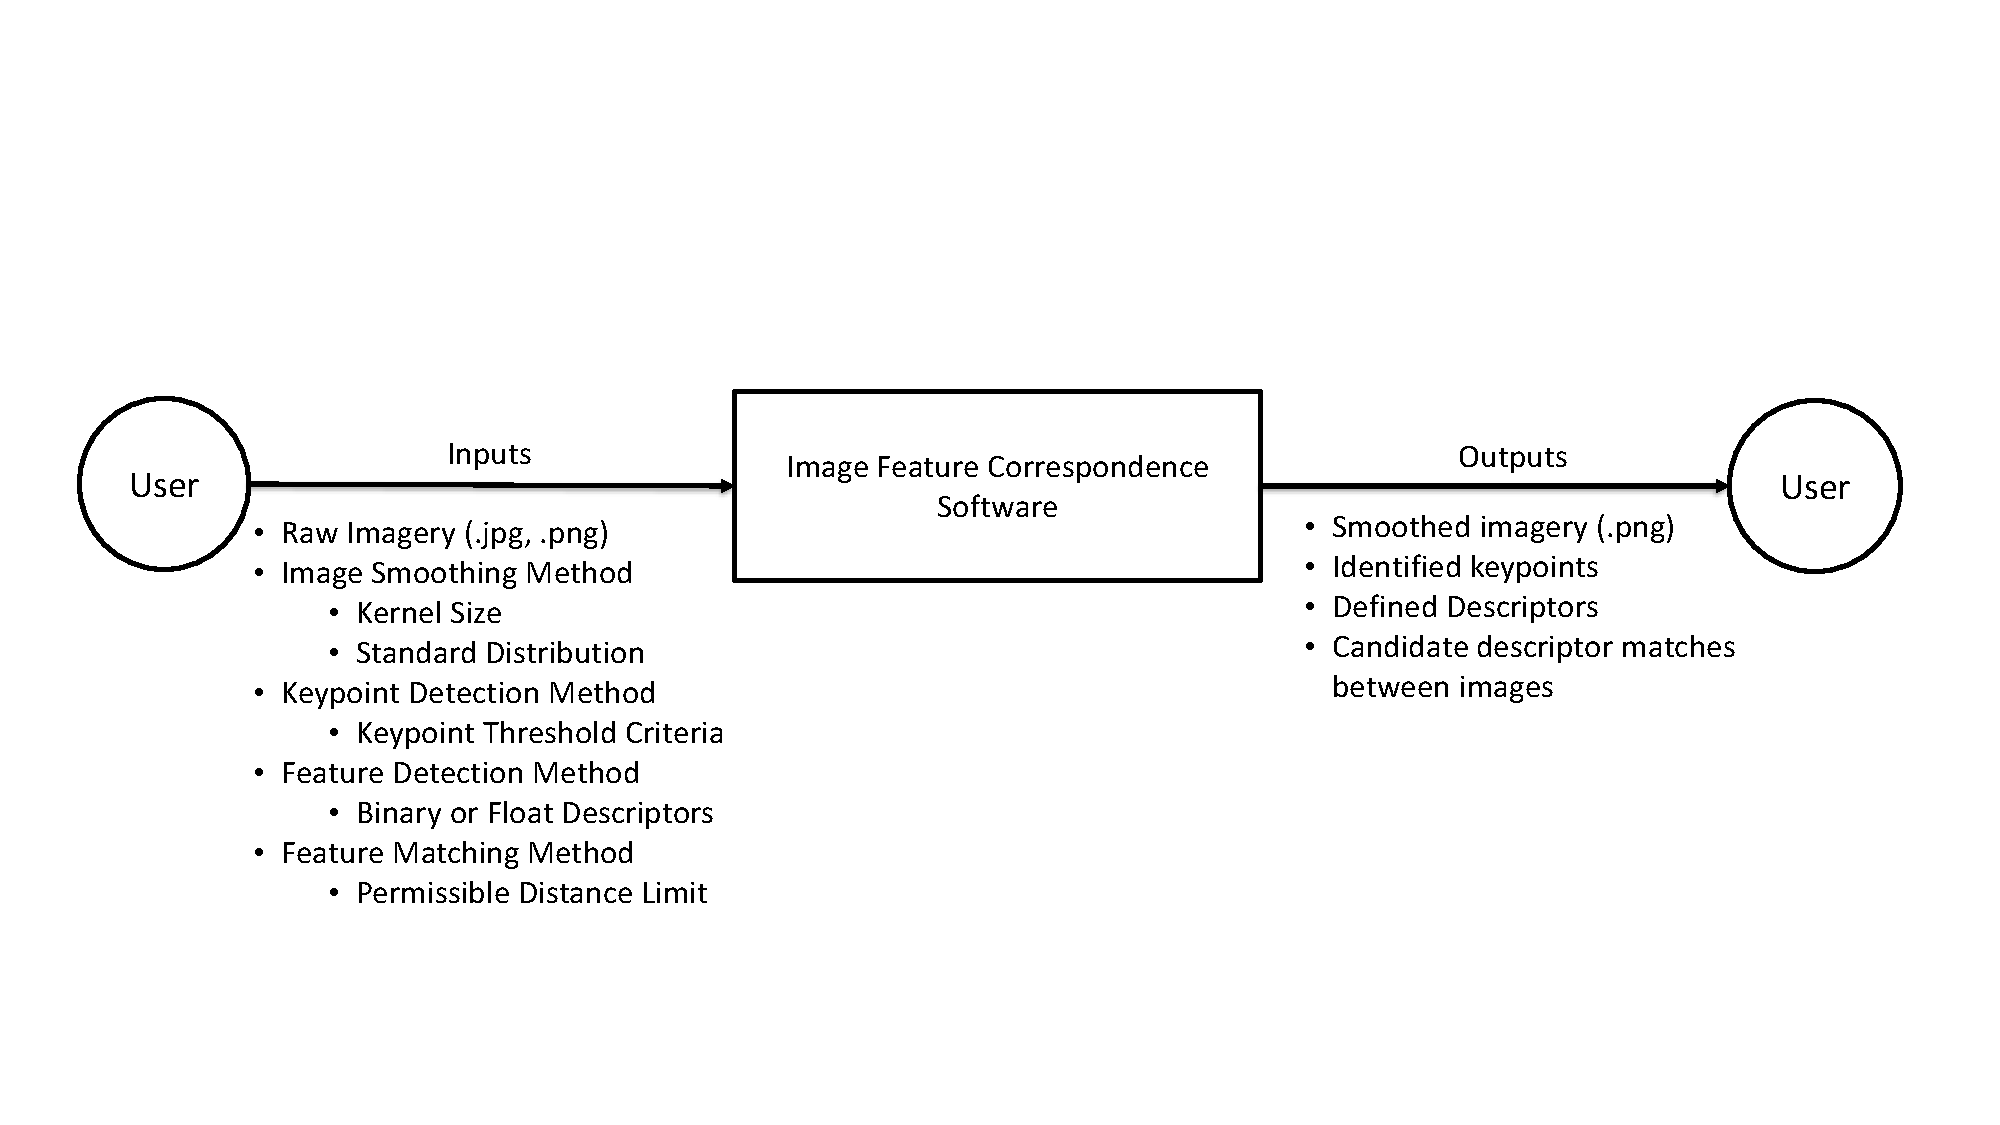
\includegraphics[width=0.6\textwidth]{SystemContextFigure}
\caption{System Context}
\label{Fig_SystemContext} 
\end{center}
\end{figure}

\begin{itemize}
\item User Responsibilities:
\begin{itemize}
\item Provide camera configuration data and imagery data to the system
\item Verify that the input data is contained in the correct data structures
\item Configure the type of feature-handler algorithms to be used with corresponding 
threshold criteria
\end{itemize}
\item \progname{} Responsibilities:
\begin{itemize}
\item Detect data type mismatch, such as a string of characters instead of a
  floating point number
\item Assess whether inputs constitute a fully defined physical setup
\item Calculate required outputs
\item Provide a quality metric of confidence in the calculated outputs
\end{itemize}
\end{itemize}

This software is not intended for use in safety-critical applications. If it is required for 
applications that are deemed to be safety-critical, then the software will need to undergo a new 
review and verification cycle.

\subsection{User Characteristics} \label{SecUserCharacteristics}
The end user of the IFC software should have an undergraduate understanding of introductory 
mechanics of robots, statistics, and computer vision algorithms.

\subsection{System Constraints}
The IFC software shall be compatible with Python 3.1 libraries, such as
OpenCV.

\section{Specific System Description}
This section first presents the problem description, which gives a high-level
view of the problem to be solved.  This is followed by the solution characteristics
specification, which presents the assumptions, theories, definitions and finally
the instance models. 

\subsection{Problem Description} \label{Sec_pd}

\progname{} is intended to evaluate how imagery data from robot-based cameras can 
can be manipulated to define and align features between separate images in support 
of downstream operations for extrinsic camera calibration.

\subsubsection{Terminology and  Definitions}

This subsection provides a list of terms that are used in the subsequent
sections and their meaning, with the purpose of reducing ambiguity and making it
easier to correctly understand the requirements:

\begin{itemize}

\item \textbf{Features:} Distinctive patterns or structures in an image that are 
identifiable and useful for matching between images

\item \textbf{Keypoints:} Specific pixel locations in an image that represent 
significant and repeatable features.

\item \textbf{Correspondences:} Pairs of keypoints between two images that represent 
represent the same real-world point.

\item \textbf{Extrinsic Parameters:} The transform between the 3D camera frame to the 
3D world frame.

\item \textbf{Intrinsic Parameters:} camera parameters that pertain to the transform of the 
2D image plane frame to the 3D camera frame.

\item \textbf{Hand-eye:} the relation between the robot end-effector to the camera frame

\item \textbf{Robot-world:} the relation between the robot base frame to the world frame

\item \textbf{Pose:} refers to the position and orientation of an object, sensor, or robot 
within a given reference frame. 

\item \textbf{Patch:} A square region of an image of an assigned size.
\end{itemize}

\subsubsection{Physical System Description} \label{sec_phySystDescrip}
The physical system of \progname{}, as shown in Figure \ref{Wang_EOH}, outlines 
case of a single-camera, single target configuration. This outlines the frames of 
interest for \ref{PS_1}. This configuration can be extrapolated to the multi-camera, 
multi-target case, as shown in \ref{OASIS}. A representation of equivalent keypoints 
between images is shown in \ref{MV_HZ}.
\\
\\
\noindent\label{PS_1}PS1: Frames for the robot base, hand, camera, and target landmark\\
\noindent\label{PS_2}PS2: Known base-to-hand transform.\\
\noindent\label{PS_3}PS3: Projected camera images from distinct camera poses.

\begin{figure}[h!]
  \begin{center}
  \centering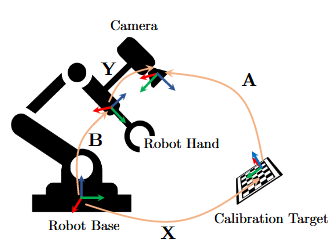
\includegraphics[width=0.5\textwidth]{Images/Wang_EOH.png}
  \caption{Single-camera robotic manipulator robot-world hand eye 
  configuration. Modified from \cite{Wang_2022}.}.
  \label{Wang_EOH}
  \end{center}
\end{figure}

\begin{figure}[ht!]
  \begin{center}
  \centering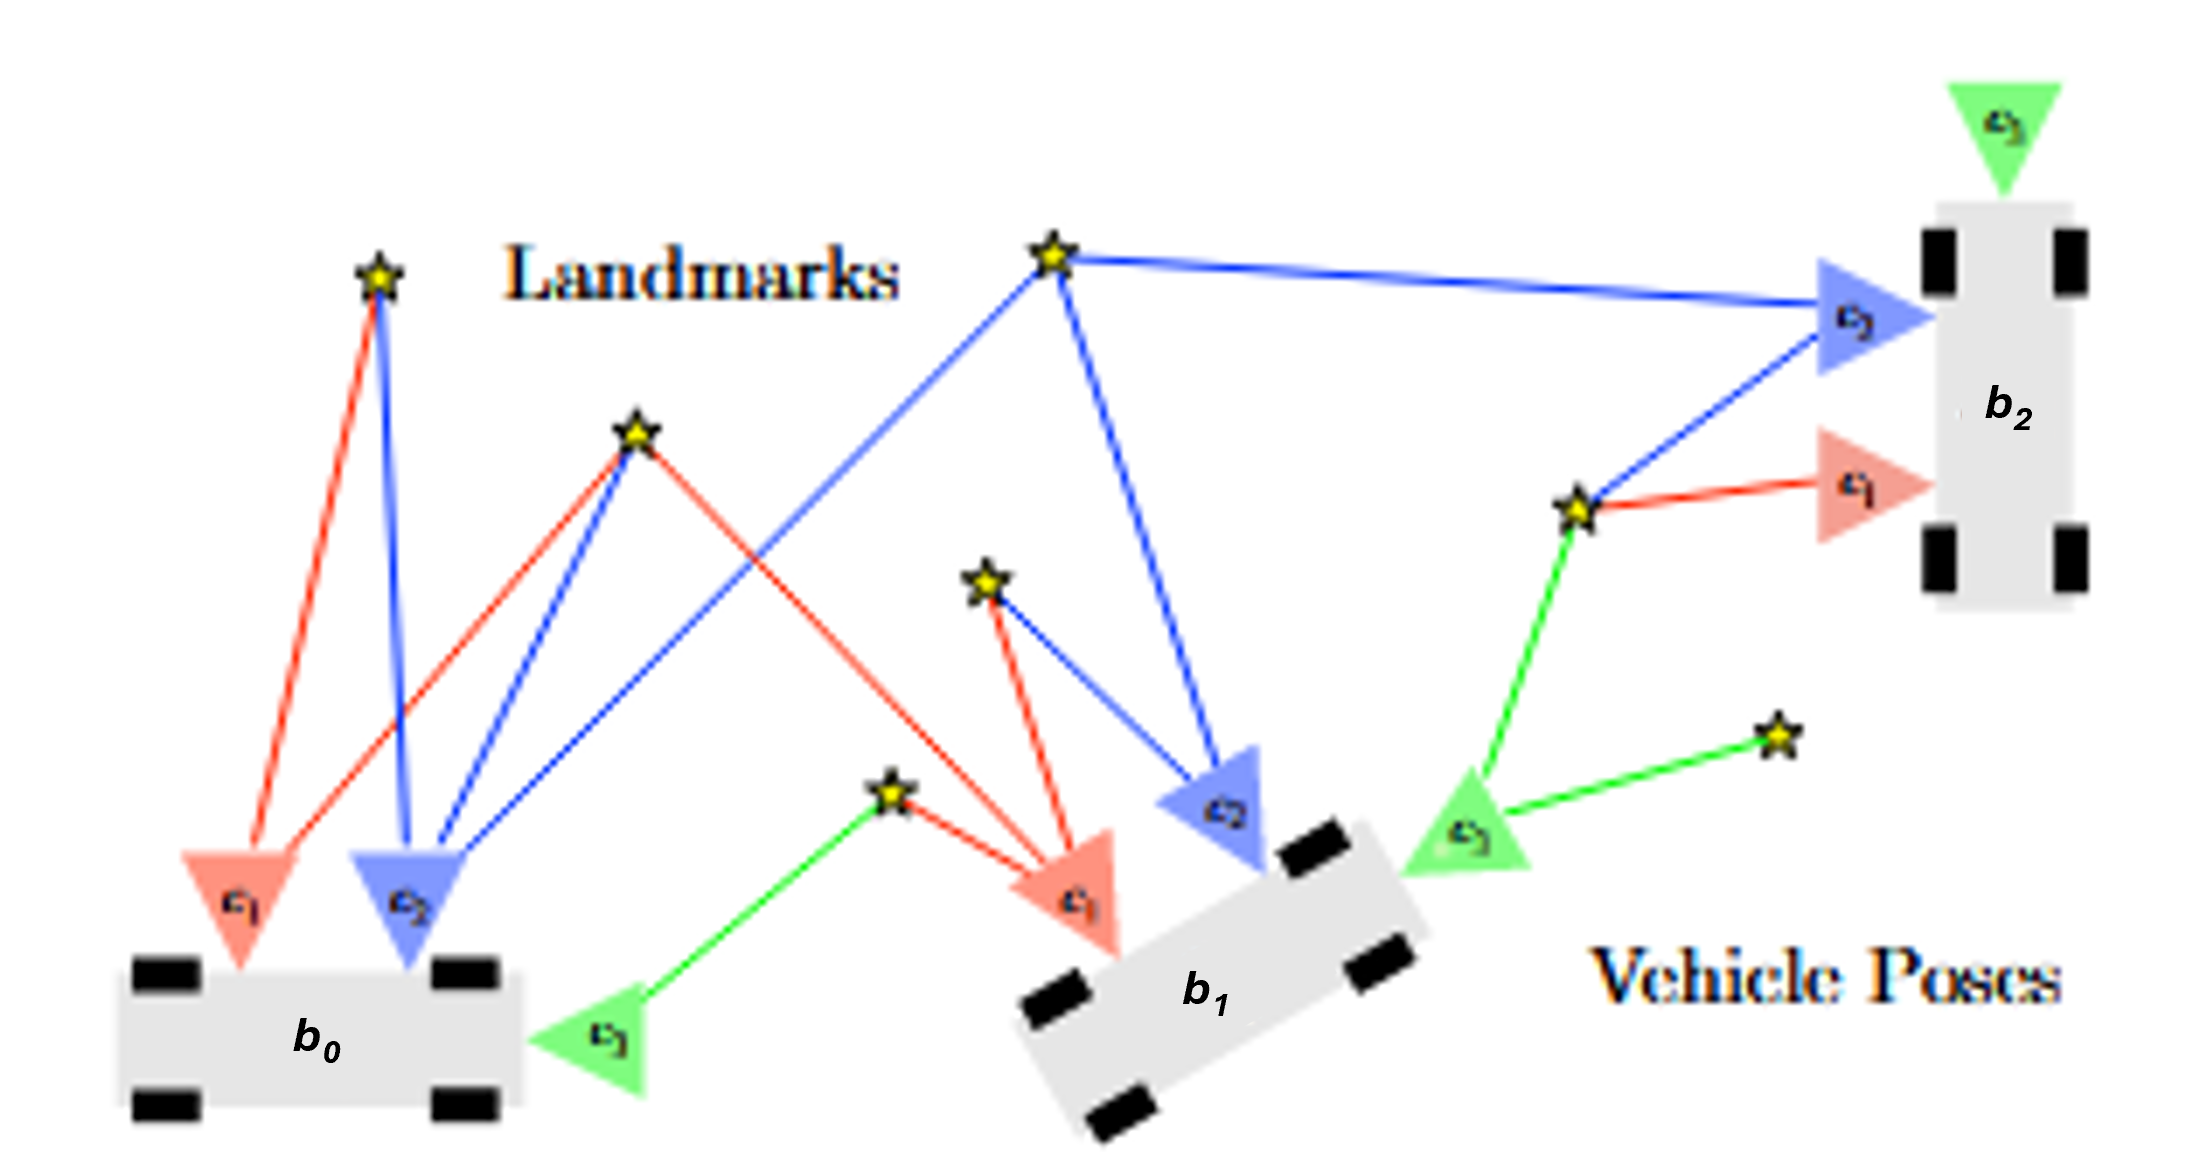
\includegraphics[width=0.5\textwidth]{Images/OASIS_RevVar.png}
  \caption{Multi-camera mobile robotic platform. 
  Modified from \cite{OASIS_2024}.}
  \label{OASIS}
  \end{center}
\end{figure}

\begin{figure}[ht!]
  \begin{center}
  \centering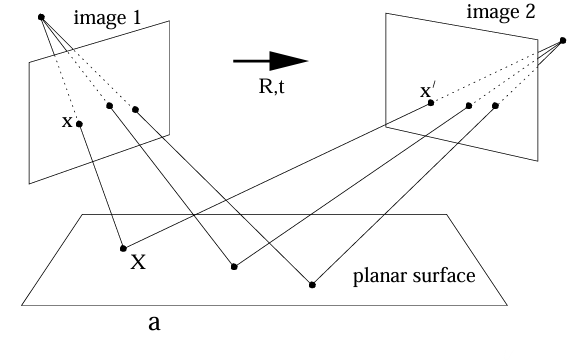
\includegraphics[width=0.5\textwidth]{Images/MULTIVIEW.png}
  \caption{Multi-camera mobile robotic platform. 
  Modified from \cite{Hartley_Zisserman}.}.
  \label{MV_HZ}
  \end{center}
\end{figure}



\subsubsection{Goal Statements}
\noindent The system goals follow.

\begin{itemize}

  \item[GS\refstepcounter{goalnum}\thegoalnum \label{define_features}:]
    Define the method(s) used to search for feature correspondences between each image frame.
    
  \item[GS\refstepcounter{goalnum}\thegoalnum \label{compare_features}:]
    Define the method(s) used to search for feature correspondences between each image frame.
  
  \item[GS\refstepcounter{goalnum}\thegoalnum \label{identify_features}:]
    Identify a collection of features from each input image frame. 
  
  \item[GS\refstepcounter{goalnum}\thegoalnum \label{identify_matches}:] 
    Identify feature correspondences amongst each input image.
  
  \item[GS\refstepcounter{goalnum}\thegoalnum \label{report_matches}:]
    Generate a report of the identified feature correspondences.
    
\end{itemize}

\subsection{Solution Characteristics Specification}
\begin{figure}[H]
  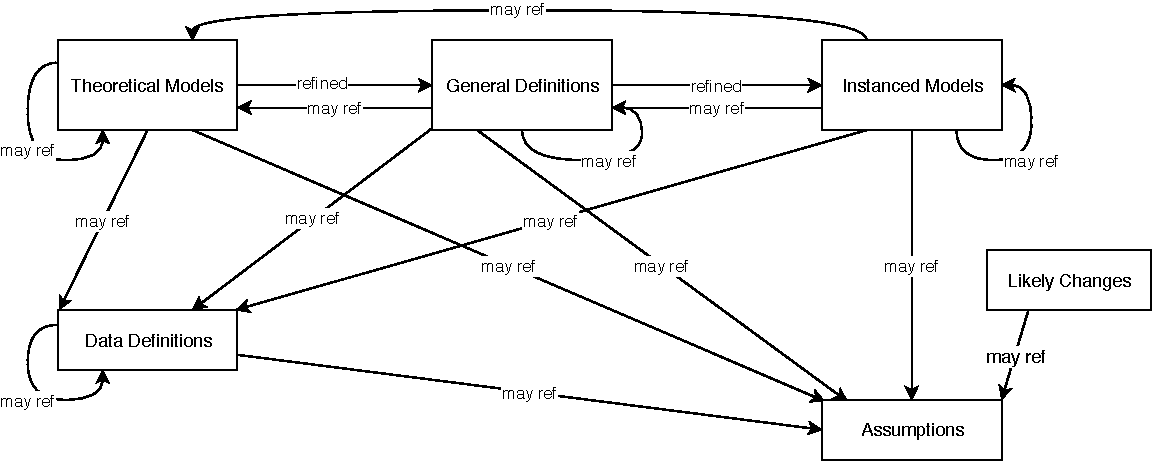
\includegraphics[scale=0.9]{RelationsBetweenTM_GD_IM_DD_A.pdf}
\end{figure}

The instance models that govern \progname{} are presented in
Subsection~\ref{sec_instance}.  The information to understand the meaning of the
instance models and their derivation is also presented, so that the instance
models can be verified.

\subsubsection{Types}
Omitted for Rev 1.0 release.

\subsubsection{Scope Decisions}
Control of the ambient illumination conditions falls outside the scope of this software.
It is the responsibility of the user to verify that the ambient lighting conditions do 
not change to a significant degree during the image capture process.


\subsubsection{Modelling Decisions}
Omitted for Rev 1.0 release.

\subsubsection{Assumptions} \label{sec_assumpt}
This section simplifies the original problem and helps in developing the
theoretical model by filling in the missing information for the physical system.
The numbers given in the square brackets refer to the theoretical model [TM],
general definition [GD], data definition [DD], instance model [IM], or likely
change [LC], in which the respective assumption is used.

\begin{itemize}
\item[A\refstepcounter{assumpnum}\theassumpnum \label{A_min_num_cameras}:]
Imagery shall be provided by at least one camera (\dref{TM_Dist_Ham}).

\item[A\refstepcounter{assumpnum}\theassumpnum \label{A_camera_model}:]
All supplied imagery is produced by a pinhole model, affine camera 
(\tref{TM_FAST}, \tref{TM_BRIEF}, \dref{GD_2D_Gauss}).

\item[A\refstepcounter{assumpnum}\theassumpnum \label{A_greyscale}:]
All imagery will be input as greyscale data (\dref{GD_2D_Gauss}).

\item[A\refstepcounter{assumpnum}\theassumpnum \label{A_RT_Memory}:]
The solution is not limited to memory constraints observed in hardware used for real-time 
applications (\tref{TM_BRIEF}).

\end{itemize}

\subsubsection{Theoretical Models}\label{sec_theoretical}
This section focuses on the general equations and laws that \progname{} is based
on.

~\newline



% Theoretical Model 1
\noindent
\begin{minipage}{\textwidth}
\renewcommand*{\arraystretch}{1.5}
\begin{tabular}{| p{\colAwidth} | p{\colBwidth}|}
\hline
\rowcolor[gray]{0.9}
Number& TM\refstepcounter{theorynum}\thetheorynum \label{TM_ND_Gauss}\\
\hline
Label &\bf N-Dimensional Gaussian Kernel \\
\hline
Equation&$G_{N-Dim}(\overrightarrow{x},\sigma) = \frac{1}{2\pi\sigma^2}e^{-\frac{\overrightarrow{x}}
{2\sigma^2}}$  \\
\hline
Description & The above equation represents the distribution of data when defined as a n-dimensional  
Gaussian Distribution. $\overrightarrow{x}$ is the collection of n-dimensions in the 
Gaussian distribution. $\sigma$ is the standard deviation of the Gaussian distribution. 
\\
\hline
Notes & All variables are unitless. \\
\hline
Source & \cite{Gauss_Kernel} \\
\hline
Ref.\ By & \dref{GD_2D_Gauss}\\
\hline
Pre-conditions for TM\thetheorynum: &None \\
\hline
Derivation for TM\thetheorynum: &None \\
\hline
\end{tabular}
\end{minipage}\\

% Theoretical Model 2
\noindent
\begin{minipage}{\textwidth}
\renewcommand*{\arraystretch}{1.5}
\begin{tabular}{| p{\colAwidth} | p{\colBwidth}|}
\hline
\rowcolor[gray]{0.9}
Number& TM\refstepcounter{theorynum}\thetheorynum \label{TM_FAST}\\
\hline
Label &\bf Features from Accelerated Segment Test (FAST)  \\
\hline
Equation& $S_{p \rightarrow x} = \begin{cases} 
  \mathit{d, , I_{p \rightarrow x} \leq I_{p} - t} \quad\textnormal{(darker)} \\
  \mathit{s, , I_{p \rightarrow x} \leq I_{p} + t} \quad\textnormal{(similar)} \\
  \mathit{b, , I_{p} + t \leq I_{p \rightarrow x} \quad\textnormal{(brighter)}} \\
  \end{cases}
$  \\
\hline
Description & For the 2D image from an pinhole, affine camera model (\aref{A_camera_model}), $\mathit{x}$ 
represents the 16 contiguous pixels that surround pixel $\mathit{p}$ within the image plane, or 
$\mathit{x} \in \{1,...,16\}$. 
$S_{p \rightarrow x}$ represents the comparison of pixel intensity for $\mathit{p}$ to $\mathit{x}$, 
with an assignment of $\mathit{d, s}$, or $\mathit{b}$ to represent that pixel $\mathit{p}$ is brighter, 
darker, or similar to its neighbours. If the pixel is classified as either a $\mathit{b}$ or a 
$\mathit{d}$, then the pixel is defined as a keypoint for edge detection. 
\\
\hline
Notes & All variables are unitless. \\
\hline
Source & \cite{FAST} \\
\hline
Ref.\ By & \dref{GD_FAST}, \lcref{LC_keypoint_method}\\
\hline
Pre-conditions for TM\thetheorynum: &None \\
\hline
Derivation for TM\thetheorynum: &None \\
\hline
\end{tabular}
\end{minipage}\\



% Theoretical Model 3
\noindent
\begin{minipage}{\textwidth}
\renewcommand*{\arraystretch}{1.5}
\begin{tabular}{| p{\colAwidth} | p{\colBwidth}|}
\hline
\rowcolor[gray]{0.9}
Number& TM\refstepcounter{theorynum}\thetheorynum \label{TM_BRIEF}\\
\hline
Label &\bf Binary Robust Independent Elementary Features (BRIEF)  \\
\hline
Equation& $\mathit{d_{k}}= \mathbf{1}({\mathit{I(p_{k})< I(q_{k})}})$
\\
\hline
Description & For a selected patch within an 2D image from a pinhole camera (\aref{A_camera_model}), \
and $\mathit{d_{k}}$ represents the kth bit in a descriptor, pixels $\mathit{p_{k}}$ 
and $\mathit{q_{k}}$ are randomly sampled. 
\\
\hline
Notes & This theory is computationally expensive and may not be suited to real-time applications 
(\aref{A_RT_Memory}). \\
\hline
Source & \cite{opencv_orb_tutorial} \\
\hline
Ref.\ By & \dref{GD_rBRIEF}, \lcref{LC_descriptor_method}\\
\hline
Pre-conditions for TM\thetheorynum: &None \\
\hline
Derivation for TM\thetheorynum: &None \\
\hline
\end{tabular}
\end{minipage}\\

~\newline

% Theoretical Model 4
\noindent
\begin{minipage}{\textwidth}
\renewcommand*{\arraystretch}{1.5}
\begin{tabular}{| p{\colAwidth} | p{\colBwidth}|}
\hline
\rowcolor[gray]{0.9}
Number& TM\refstepcounter{theorynum}\thetheorynum \label{TM_Dist_Ham}\\
\hline
Label &\bf Hamming Distance  \\
\hline
Equation& $\mathit{d_{Hamming}(d_{k,\alpha}, d_{k,\beta}) =\sum_{i=0}^{n-1}(d_{k,\alpha} 
\bigoplus d_{k,\beta})} $ \\
\hline
Description & The Hamming distance is used to compare two binary numbers by each succesive bit, 
and return the sum, $\mathit{d_{Hamming}}$, for the binary descriptors $\mathit{\alpha}$ and 
$\mathit{\beta}$. The Hamming Distance does not represent a physical distance.
represent a physical distanced$\mathit{i}$ represents the index within the total of $\mathit{n}$ descriptors. 
$\bigoplus$ represents the bitwise exclusive-OR (XOR) operation. 
Both descriptors are assumed to originate from separate images (\aref{A_min_num_cameras}).
\\
\hline
Notes & All variables are unitless. \\
\hline
Source & \cite{opencv_flann_matcher} \\
\hline
Ref.\ By & \iref{IM_Dist_Hamm}, \lcref{LC_comparison_method}\\
\hline
Pre-conditions for TM\thetheorynum: &None \\
\hline
Derivation for TM\thetheorynum: &None \\
\hline
\end{tabular}
\end{minipage}\\

~\newline

\subsubsection{General Definitions}\label{sec_gendef}
This section collects the laws and equations that will be used in building the
instance models.

~\newline

% General Defintion 1
\noindent
\begin{minipage}{\textwidth}
\renewcommand*{\arraystretch}{1.5}
\begin{tabular}{| p{\colAwidth} | p{\colBwidth}|}
\hline
\rowcolor[gray]{0.9}
Number& GD\refstepcounter{defnum}\thedefnum \label{GD_2D_Gauss}\\
\hline
Label &\bf 2-Dimensional Gaussian Kernel \\
\hline
% Units&$MLt^{-3}T^0$\\
% \hline
SI Units&Unitless\\
\hline
Equation&$G_{2D}(u,v,\sigma) = \frac{1}{2\pi\sigma^2}e^{-\frac{u^{2} + v^{2}}
{2\sigma^2}}$  \\
\hline
Description & $G_{2D}$ represents the gaussian kernel transform that is  applied 
    to the 2D greyscale image (\aref{A_camera_model}, \aref{A_greyscale}) given by horizonal pixel $u$ and vertical pixel $v$, both of which are 
    unitless. $\sigma$ represents the allowable standard deviation of the two dimensional 
    distribution for a given image. The Gaussian kernel is used to smooth an image to reduce 
    noise amongst the individual pixels. 
\\
 & $\overrightarrow{x}$ is the collection of n-dimensions in the Gaussian distribution. 
\\
 & $\sigma$ is the standard deviation of the Gaussian distribution.
\\
\hline
  Source & TM\ref{TM_ND_Gauss} \\
  \hline
  Ref.\ By & \iref{IM_GK}\\
  \hline
\end{tabular}
\end{minipage}\\

~\newline

% General Defintion 2
\noindent
\begin{minipage}{\textwidth}
\renewcommand*{\arraystretch}{1.5}
\begin{tabular}{| p{\colAwidth} | p{\colBwidth}|}
\hline
\rowcolor[gray]{0.9}
Number& GD\refstepcounter{defnum}\thedefnum \label{GD_FAST}\\
\hline
Label &\bf FAST Implementation \\
\hline
Units&Unitless\\
\hline
Equation&$\mathit{\sum\limits_{k \in x} (|I_{k} - I(u,v)|>t) \geq N}$  \\
\hline
Description &  The threshold count of $\mathit{x \in \{1 \dots 16 \}}$ is concretely defined as $\mathit{N}$. 
$\mathit{I(u,v)}$ represents the pixel intensity of pixel $\mathit{p}$. $\mathit{I_{k}}$ represents 
the grayscale image intensity of the $k^{th}$ pixel in the circle around pixel $\mathit{p}$. 
$\mathit{t}$ represents the user-defined threshold to define an allowable range of pixel intensity.
\\
\hline
  Source & TM\ref{TM_FAST} \\
  \hline
  Ref.\ By & \iref{IM_GK}\\
  \hline
\end{tabular}
\end{minipage}\\



% General Defintion 3
\noindent
\begin{minipage}{\textwidth}
\renewcommand*{\arraystretch}{1.5}
\begin{tabular}{| p{\colAwidth} | p{\colBwidth}|}
\hline
\rowcolor[gray]{0.9}
Number& GD\refstepcounter{defnum}\thedefnum \label{GD_rBRIEF}\\
\hline
Label &\bf Rotated Brief \\
\hline
% Units&$MLt^{-3}T^0$\\
% \hline
Units&Unitless\\
\hline
Equation&$d_{k} = I(p_{k}^{'}) < I(q_{k}^{'})$  \\
\hline
Description & For a defined patch size around a selected keypoint, pixels $\mathit{p}$ and 
$\mathit{q}$ are randomly selected. $\mathit{d_{k}}$ represents the kth bit in a descriptor, 
pixels $\mathit{p_{k}^{'}}$ and $\mathit{q_{k}^{'}}$ are randomly sampled. This ensures that 
BRIEF can be implemented in a manner that is rotation invariant to an image within a plane.\\
\hline
  Source & \cite{opencv_orb_tutorial} \\
  \hline
  Ref.\ By & \iref{IM_BRIEF_Desc}\\
  \hline
\end{tabular}
\end{minipage}\\




\subsubsection*{Detailed derivation of Rotated Brief Transform}
$\mathit{p_{k}}$ and $\mathit{q_{k}}$ are calculated by successive increments of a 12\textdegree. 
The transform between $\mathit{p_{k}^{'}}$ and $\mathit{q_{k}^{'}}$ is outlined below, where $\theta$ 
represents the increase in rotation by a denomination of 12\textdegree. \\

\[
\begin{bmatrix} p_k' \\ q_k' \end{bmatrix} =
\begin{bmatrix} \cos\theta & -\sin\theta \\ \sin\theta & \cos\theta \end{bmatrix}
\begin{bmatrix} p_k \\ q_k \end{bmatrix}
\]

\subsubsection{Data Definitions}\label{sec_datadef}
\textcolor{red}{\textbf{No data definitions are outlined for the current release.}}

\subsubsection{Instance Models} \label{sec_instance}    
This section transforms the problem defined in Section~\ref{Sec_pd} into 
one which is expressed in mathematical terms. It uses concrete symbols defined 
in Section~\ref{sec_datadef} to replace the abstract symbols in the models 
identified in Sections~\ref{sec_theoretical} and~\ref{sec_gendef}.

~\newline

%Instance Model 1
\noindent
\begin{minipage}{\textwidth}
\renewcommand*{\arraystretch}{1.5}
\begin{tabular}{| p{\colAwidth} | p{\colBwidth}|}
  \hline
  \rowcolor[gray]{0.9}
  Number& IM\refstepcounter{instnum}\theinstnum \label{IM_GK}\\
  \hline
  Label& \bf Gaussian-Smoothed Image, $\mathit{\mathcal{I'}_{i, j}(u,v, \sigma)}$\\
  \hline
  Input&$\mathit{\mathcal{I}_{i, j}(u,v)}$, $\sigma$ from \dref{GD_2D_Gauss}\\
  \hline
  Output&$\mathit{\mathcal{I'}_{i, j}(u,v, \sigma)}$ from \tref{TM_ND_Gauss} \\
  \hline
  Description&$\mathit{\mathcal{I'}_{i, j}(u,v, \sigma)}$ is the smoothed output image.\\
  &$\mathit{\mathcal{I}_{i, j}(u,v, \sigma)}$ is the unfiltered input image.\\
  &$\sigma$ is the standard deviation of the 2D Gaussian Distribution.\\
  \hline
  Sources& \cite{Gauss_Kernel} \\
  \hline
  Ref.\ By & \gsref{identify_features}, \gsref{identify_matches},\iref{IM_FAST_Detect}\\
  \hline
\end{tabular}
\end{minipage}\\

~\newline

% Instance Model 2
\noindent
\begin{minipage}{\textwidth}
\renewcommand*{\arraystretch}{1.5}
\begin{tabular}{| p{\colAwidth} | p{\colBwidth}|}
  \hline
  \rowcolor[gray]{0.9}
  Number& IM\refstepcounter{instnum}\theinstnum \label{IM_FAST_Detect}\\
  \hline
  Label& \bf Image Keypoint Detection, $\mathit{\mathcal{D}_{i, j}(u,v)}$\\
  \hline
  Input&$\mathit{\mathcal{I}_{i, j}(u,v, \sigma)}$ from \iref{IM_GK}, $t$ \\
  \hline
  Output&$\mathit{\mathcal{D}_{i, j}(u,v)}$, such that D is an n-dimensional 2D matrix of the horizontal 
  and vertical pixel coordinates in the form of (u,v).\\
  \hline
  Description& $\mathit{\mathcal{D}_{i, j}(u,v)}$ defined by the mapping transform, $S_{p \rightarrow x}$, 
  as outlined in \tref{TM_FAST}.\\
  & $\mathit{\mathcal{I}_{i, j}(u,v, \sigma)}$ is the smoothed image (m x n) from \iref{IM_GK}.\\
  & $t$ is the pixel intensity threshold.\\
  \hline
  Sources& \cite{FAST} \\
  \hline
  Ref.\ By & \gsref{define_features}, \gsref{identify_features}, \iref{IM_BRIEF_Desc}\\
  \hline
\end{tabular}
\end{minipage}\\

~\newline

% Instance Model 3
\noindent
\begin{minipage}{\textwidth}
\renewcommand*{\arraystretch}{1.5}
\begin{tabular}{| p{\colAwidth} | p{\colBwidth}|}
  \hline
  \rowcolor[gray]{0.9}
  Number& IM\refstepcounter{instnum}\theinstnum \label{IM_BRIEF_Desc}\\
  \hline
  Label& \bf Produce Feature Descriptors, $\mathit{D_{bin}}$\\
  \hline
  Input&$\mathit{\mathcal{D}_{i, j}(u,v)}$ from \iref{IM_FAST_Detect}, $p_{s}$, $l_{bin}$ \\
  \hline
  Output&$\mathit{D_{bin}}$ as as variable size vector\\
  \hline
  Description&$\mathit{\mathcal{D}_{i, j}}$ is the vector of pixels (u,v) of identified keypoints, per \iref{IM_FAST_Detect}.\\
  &$p_{s}$ is the size of pixel patch to draw samples, as an integer.\\
  &$l_{bin}$ is the size of the binary descriptor, in bits, per \tref{TM_BRIEF}.\\
  &$\mathit{D_{bin}}$ is the output vector of identified descriptors, per \tref{TM_BRIEF}.\\
  \hline
  Sources& \cite{opencv_orb_tutorial} \\
  \hline
  Ref.\ By & \gsref{compare_features}, \gsref{identify_matches}, \iref{IM_Dist_Hamm}\\
  \hline
\end{tabular}
\end{minipage}\\

~\newline

% Instance Model 4
\noindent
\begin{minipage}{\textwidth}
\renewcommand*{\arraystretch}{1.5}
\begin{tabular}{| p{\colAwidth} | p{\colBwidth}|}
  \hline
  \rowcolor[gray]{0.9}
  Number& IM\refstepcounter{instnum}\theinstnum \label{IM_Dist_Hamm}\\
  \hline
  Label& \bf Inter-Image Descriptor Comparison, $\mathit{dist_{Hamming}}$\\
  \hline
  Input&$\mathit{d_{a}}$, $\mathit{d_{b}}$ from \iref{IM_BRIEF_Desc}\\
  \hline
  Output&$\mathit{dist_{Hamming}}$\\
  \hline
  Description&$\mathit{dist_{Hamming}}$ is the sum of bitwise $\mathbf{XOR}$ binary descriptors as outlined in \tref{GD_rBRIEF}.\\
  &$\mathit{d_{a}}$, $\mathit{d_{b}}$ are binary descriptors as defined by \iref{IM_BRIEF_Desc}.\\
  \hline
  Sources& \cite{opencv_flann_matcher} \\
  \hline
  Ref.\ By & \gsref{identify_matches}, \gsref{report_matches} \\
  \hline
\end{tabular}
\end{minipage}\\



\subsubsection{Input Data Constraints} \label{sec_DataConstraints}    

Table~\ref{TblInputVar} shows the data constraints on the input output
variables.  The column for physical constraints gives the physical limitations
on the range of values that can be taken by the variable.  The column for
software constraints restricts the range of inputs to reasonable values.  The
software constraints will be helpful in the design stage for picking suitable
algorithms.  The constraints are conservative, to give the user of the model the
flexibility to experiment with unusual situations.  The column of typical values
is intended to provide a feel for a common scenario.  The uncertainty column
provides an estimate of the confidence with which the physical quantities can be
measured.  This information would be part of the input if one were performing an
uncertainty quantification exercise.

The specification parameters in Table~\ref{TblInputVar} are listed in
Table~\ref{TblSpecParams}.

\begin{table}[!h]
  \caption{Input Variables} \label{TblInputVar}
  \renewcommand{\arraystretch}{1.2}
\noindent \begin{longtable*}{l l l l c} 
  \toprule
  \textbf{Var} & \textbf{Physical Constraints} & \textbf{Software Constraints} &
                             \textbf{Typical Value} & \textbf{Uncertainty}\\
  \midrule 
  $\mathit{\mathcal{I}_{i, j}(u,v)}$ & N/A & $0 \leq \mathit{\mathcal{I}_{i, j}(u,v)} \leq 255$ 
  & N/A & N/A  % at least one camera
  \\
  $\sigma$ & $\sigma > 0$ & $\sigma > 0 $ & 0.05 & N/A % std dev > 0
  \\
  $i$ & $ 1 \i > 1$ & $\leq i \leq 250$ & 40 & N/A
  \\
  $j_{max}$ & $1 \leq j_{max} \leq 10$ & $1 \leq j \leq 10$ & 3 & N/A
  \\
  \bottomrule
\end{longtable*}
\end{table}
\noindent 
\begin{description}
\item[(*)] $\mathit{\mathcal{I}_{i, j}(u,v)}$ is limited to being an 8-bit unsigned integer
\item[(*)] standard deviation, $\sigma$, is constrained to be positive and real
\item[(*)] the robot pose, $i$, must be greater than 1, but should be no greater than 250 
to avoid excessive runtimes
\item[(*)] the total number of cameras, $j_{max}$, should not exceed 10 as this exceeds the 
expected operational needs of the system
\end{description}

\subsubsection{Properties of a Correct Solution} \label{sec_CorrectSolution}

\noindent
A correct solution must exhibit high recall. Recall can be described by the comparison of true positive (TP) over the 
total predicted results, which is the sum of all true positive and false negative (FN) outcomes. A specific performance metric 
may be assigned [LC5000].

$$Recall = \frac{TP}{TP + FN}$$



\noindent
\\
\\
\textcolor{red}{\textbf{This table should be addressed for a subsequent revision. As it standard, there are currently no 
identified physical constraints on the system.}}
\begin{table}[!h]
\caption{Output Variables} \label{TblOutputVar}
\renewcommand{\arraystretch}{1.2}
\noindent \begin{longtable*}{l l} 
  \toprule
  \textbf{Var} & \textbf{Physical Constraints} \\
  \midrule 

  \\
  \bottomrule
\end{longtable*}
\end{table}

\section{Requirements}
This section provides the functional requirements, the business tasks that the
software is expected to complete, and the nonfunctional requirements, the
qualities that the software is expected to exhibit.

\newpage
\subsection{Functional Requirements}

\noindent \begin{itemize}

% Inputs
\item[R\refstepcounter{reqnum}\thereqnum \label{R_Update_SD}:] The IFC software shall accept 
updates to the variance in image noise,  $\mathit{\sigma}$, upon user input.

\item[R\refstepcounter{reqnum}\thereqnum \label{R_Update_Intensity}:] The IFC software shall accept 
updates to the image intensity threshold, $\mathit{t}$, upon user input.

\item[R\refstepcounter{reqnum}\thereqnum \label{R_Update_Patch}:] The IFC software shall accept 
updates to the patch size, $\mathit{p_{s}}$, upon user input.

\item[R\refstepcounter{reqnum}\thereqnum \label{R_Update_BinSize}:] The IFC software shall accept 
updates to the bin size, $\mathit{l_{bin}}$, upon user input.

\item[R\refstepcounter{reqnum}\thereqnum \label{R_Default_Noise}:] The IFC software shall use the 
default noise suppresion parameters if no option is specified by the user.

\item[R\refstepcounter{reqnum}\thereqnum \label{R_Default_FD}:] The IFC software shall use the 
default feature detection method if no option is specified by the user.

\item[R\refstepcounter{reqnum}\thereqnum \label{R_Default_KD}:] The IFC software shall use the 
default keypoint descriptor method if no option is specified by the user.

\item[R\refstepcounter{reqnum}\thereqnum \label{R_Default_FM}:] The IFC software shall use the 
default descriptor matching method if no option is specified by the user.

% Calculations 
\item[R\refstepcounter{reqnum}\thereqnum \label{R_NoiseReduction}:] The IFC software shall 
implement noise reduction on an input greyscale image per a prescribed standard deviation (from 
\iref{IM_GK}).

\item[R\refstepcounter{reqnum}\thereqnum \label{R_DetectKeypoints}:] The IFC software shall, given a 2D 
greyscale image, define a set of keypoints per the alloted threshold criteria (from 
\iref{IM_FAST_Detect}).

\item[R\refstepcounter{reqnum}\thereqnum \label{R_DefineDescriptors}:] The IFC software shall 
define feature descriptors from identified keypoints (from \iref{IM_BRIEF_Desc})..

\item[R\refstepcounter{reqnum}\thereqnum \label{R_CompareDescriptors}:] The IFC software shall 
identify matches between descriptors that originate from separate images (from \iref{IM_Dist_Hamm}).

% Outputs 
\item[R\refstepcounter{reqnum}\thereqnum \label{R_OutputCorrespondences}:] The IFC software shall 
provide a .csv file that outlines the respective feature matches.

% Verify Outputs
\item[R\refstepcounter{reqnum}\thereqnum \label{R_DistinctImages}:] The IFC software shall verify 
that all features are matched to features that originate from separate images.

\item[R\refstepcounter{reqnum}\thereqnum \label{R_UniqueMatch_IDs}:] The IFC software shall verify 
that all feature correspondences are uniquely defined by the two respective sets of cameras, image frame, 
and associated pixels.

\end{itemize}

\subsection{Nonfunctional Requirements}

\noindent \begin{itemize}

\item[NFR\refstepcounter{nfrnum}\thenfrnum \label{NFR_Usability}:] \textbf{Usability}
  The IFC software shall be compatible with Python 3.1 libraries, such as OpenCV.

\end{itemize}

\subsection{Rationale}

The scope and assumptions of this document are intended to encapsulate a realistic problem formulation 
software. This software is intended for use in laboratory experimentation and configurations, rather than 
as an off-the-shelf product for applications that involve more risk, such as those that are safety-critical 
or mission critical in scope.

\section{Likely Changes}    

\noindent \begin{itemize}

\item[LC\refstepcounter{lcnum}\thelcnum\label{LC_keypoint_method}:] 
The theoretical model of keypoint detection will be abstracted to expand the types of 
implementation models that can be used.

\item[LC\refstepcounter{lcnum}\thelcnum\label{LC_descriptor_method}:] 
The theoretical model of assigning feature descriptors will be abstracted to expand the types of 
implementation models that can be used.

\item[LC\refstepcounter{lcnum}\thelcnum\label{LC_comparison_method}:] 
The theoretical model of descriptor matching will be abstracted to expand the types of 
implementation models that can be used.

\end{itemize}

\section{Unlikely Changes}    

\noindent \begin{itemize}

\item[LC\refstepcounter{lcnum}\thelcnum\label{RGB_Data}:] It is unlikely that the design 
will need to be adjusted to perform computation on RGB data instead of grayscale data.

\end{itemize}

\section{Traceability Matrices and Graphs}

The purpose of the traceability matrices is to provide easy references on what
has to be additionally modified if a certain component is changed.  Every time a
component is changed, the items in the column of that component that are marked
with an ``X'' may have to be modified as well.  Table~\ref{Table:trace} shows the
dependencies of theoretical models, general definitions, data definitions, and
instance models with each other. Table~\ref{Table:R_trace} shows the
dependencies of instance models, requirements, and data constraints on each
other. Table~\ref{Table:A_trace} shows the dependencies of theoretical models,
general definitions, data definitions, instance models, and likely changes on
the assumptions.

\afterpage{
\begin{landscape}
\begin{table}[h!]
\centering
\begin{tabular}{|c|c|c|c|c|c|c|c|c|c|c|c|c|c|c|c|c|c|c|c|}
\hline
	& \aref{A_min_num_cameras}& \aref{A_camera_model}& \aref{A_greyscale}& \aref{A_RT_Memory}\\
\hline
\tref{TM_ND_Gauss}              & & &X& \\ \hline
\tref{TM_FAST}                  & &X& & \\ \hline
\tref{TM_BRIEF}                 & &X& &X\\ \hline
\tref{TM_Dist_Ham}              &X& & & \\ \hline 
\dref{GD_2D_Gauss}              & &X& & \\ \hline
\dref{GD_FAST}                  & & & & \\ \hline
\dref{GD_rBRIEF}                & & & & \\ \hline
\iref{IM_GK}                    & & & & \\ \hline
\iref{IM_FAST_Detect}           & & & & \\ \hline
\iref{IM_BRIEF_Desc}            & & & & \\ \hline
\iref{IM_Dist_Hamm}             & & & & \\ \hline
\lcref{LC_keypoint_method}      & & & & \\ \hline
\lcref{LC_descriptor_method}    & & & & \\ \hline
\lcref{LC_comparison_method}    & & & & \\ \hline
\hline
\end{tabular}
\caption{Traceability Matrix Showing the Connections Between Assumptions and Other Items}
\label{Table:A_trace}
\end{table}
\end{landscape}
}

\begin{landscape}
\begin{table}[h!]
\centering
\begin{tabular}{|c|c|c|c|c|c|c|c|c|c|c|c|c|c|c|}
\hline        
& \tref{TM_ND_Gauss}& \tref{TM_FAST}& \tref{TM_BRIEF}& \tref{TM_Dist_Ham}& 
\dref{GD_2D_Gauss} & \dref{GD_FAST}  & \dref{GD_rBRIEF} &
\iref{IM_GK} & \iref{IM_FAST_Detect}& \iref{IM_BRIEF_Desc}& \iref{IM_Dist_Hamm}&
\lcref{LC_keypoint_method} & \lcref{LC_descriptor_method} & \lcref{LC_comparison_method}\\
\hline
\tref{TM_ND_Gauss}              & & & & &X& & &X& & & & & & \\ \hline
\tref{TM_FAST}                  & & & & & &X& & &X& & &X& & \\ \hline
\tref{TM_BRIEF}                 & & & & & & &X& & &X& & &X& \\ \hline
\tref{TM_Dist_Ham}              & & & & & & & & & & &X& & &X\\ \hline
\dref{GD_2D_Gauss}              & & & & & & & &X& & & & & & \\ \hline
\dref{GD_FAST}                  & & & & & & & & &X& & & & & \\ \hline
\dref{GD_rBRIEF}                & & & & & & & & & &X& & & & \\ \hline
\iref{IM_GK}                    & & & & & & & & &X& & & & & \\ \hline
\iref{IM_FAST_Detect}           & & & & & & & & & &X& & & & \\ \hline
\iref{IM_BRIEF_Desc}            & & & & & & & & & & &X& & & \\ \hline
\iref{IM_Dist_Hamm}             & & & & & & & & & & & & & & \\ \hline
\lcref{LC_keypoint_method}      & & & & & &X& & &X& & & & & \\ \hline
\lcref{LC_descriptor_method}    & & & & & & &X& & &X& & & & \\ \hline
\lcref{LC_comparison_method}    & & & & & & & & & & &X& & & \\ \hline
\hline
\end{tabular}
\caption{Traceability Matrix Showing the Connections Between Items of Different Sections}
\label{Table:trace}
\end{table}
\end{landscape}




\begin{landscape}
\begin{table}[h!]
\centering
\begin{tabular}{|c|c|c|c|c|c|c|c|c|c|c|c|c|c|c|c|c|c|c|c|c|c|c|}
\hline
	& \iref{IM_GK} & \iref{IM_FAST_Detect}& \iref{IM_BRIEF_Desc}& \iref{IM_Dist_Hamm}
  & \rref{R_Update_SD} &\rref{R_Update_Intensity} &\rref{R_Update_Patch} &\rref{R_Update_BinSize}
  & \rref{R_Default_Noise} &\rref{R_Default_FD} & \rref{R_Default_KD} 
  & \rref{R_Default_FM} &\rref{R_NoiseReduction}  &\rref{R_DetectKeypoints} 
  & \rref{R_DefineDescriptors} &\rref{R_CompareDescriptors} &\rref{R_OutputCorrespondences}
  & \rref{R_DistinctImages} &\rref{R_UniqueMatch_IDs} \\
\hline
                              % I1I2I3I4 1 2 3 4 5 6 7 8 9 101112131415
\iref{IM_GK}                    & &X& & &X& & & &X& & & &X& & & & & & \\ \hline
\iref{IM_FAST_Detect}           & & &X& & &X& & & &X& & & &X& & & & & \\ \hline
\iref{IM_BRIEF_Desc}            & & & &X& & &X&X& & &X& & & &X& & & & \\ \hline
\iref{IM_Dist_Hamm}             & & & & & & & & & & & &X& & & &X&X&X&X\\ \hline
\rref{R_Update_SD}              &X& & & & & & & & & & & &X& & & & & & \\ \hline
\rref{R_Update_Intensity}       & &X& & & & & & & & & & & &X& & & & & \\ \hline
\rref{R_Update_Patch}           & & &X& & & & & & & & & & & &X& & & & \\ \hline
\rref{R_Update_BinSize}         & & &X& & & & & & & & & & & &X& & & & \\ \hline
\rref{R_Default_Noise}          & & & & & & & & & & & & &X& & & & & & \\ \hline
\rref{R_Default_FD}             &X& & & & & & & & & & & & &X& & & & & \\ \hline
\rref{R_Default_KD}             & &X& & & & & & & & & & & & &X& & & & \\ \hline
\rref{R_Default_FM}             & & &X& & & & & & & & & & & & &X& & & \\ \hline
\rref{R_NoiseReduction}         &X& & & & & & & & & & & &X& & & & & & \\ \hline
\rref{R_DetectKeypoints}        & &X& & & & & & & & & & & & & & & & & \\ \hline
\rref{R_DefineDescriptors}      & & &X& & & & & & & & & & & & & & & & \\ \hline
\rref{R_CompareDescriptors}     & & & &X& & & & & & & & & & & & & & & \\ \hline
\rref{R_OutputCorrespondences}  & & & &X& & & & & & & & & & & & & & & \\ \hline
\rref{R_DistinctImages}         & & & &X& & & & & & & & & & & & & & & \\ \hline
\rref{R_UniqueMatch_IDs}        & &X&X&X& & & & & & & & & & & & & & & \\ \hline
\hline
\end{tabular}
\caption{Traceability Matrix Showing the Connections Between Requirements and Instance Models}
\label{Table:R_trace}
\end{table}
\end{landscape}

\section{Development Plan}
\textcolor{red}{\textbf{This section may be expanded upon as part of a future release.}}

\section{Values of Auxiliary Constants}
\textcolor{red}{\textbf{No auxillary constants are defined for this software.}}

\newpage

\bibliographystyle {plainnat}
\bibliography {../../refs/References}

\newpage
\textbf{\\ \\ End of Document.}
\end{document}